\documentclass{ieeeaccess}
\usepackage{cite}
\usepackage{amsmath,amssymb,amsfonts}
\usepackage{array}
\usepackage{booktabs}
\usepackage{graphicx}
\usepackage{textcomp}
\usepackage{tabularx}
\usepackage{xcolor}
\usepackage{url}
\usepackage{hyperref}
\hypersetup{hidelinks}
\graphicspath{{figures/}}
% Generated from artifacts/raw CSV outputs; do not hand edit.
\newcommand{\FEVERDensePrecision}{0.849}
\newcommand{\FEVERDenseRecall}{1.000}
\newcommand{\FEVERDenseFOne}{0.896}
\newcommand{\FEVERDenseRephrase}{1.000}
\newcommand{\FEVERDenseComposable}{0.659}
\newcommand{\FEVERDenseSourceFOne}{0.152}
\newcommand{\FEVERLexicalPrecision}{0.987}
\newcommand{\FEVERLexicalRecall}{1.000}
\newcommand{\FEVERLexicalFOne}{0.992}
\newcommand{\FEVERLexicalRephrase}{1.000}
\newcommand{\FEVERLexicalComposable}{0.660}
\newcommand{\FEVERLexicalSourceFOne}{0.152}
\newcommand{\FEVERXProvPrecision}{0.879}
\newcommand{\FEVERXProvRecall}{1.000}
\newcommand{\FEVERXProvFOne}{0.917}
\newcommand{\FEVERXProvRephrase}{1.000}
\newcommand{\FEVERXProvComposable}{0.660}
\newcommand{\FEVERXProvSourceFOne}{0.152}
\newcommand{\FEVERN}{19998}
\newcommand{\SciFactDensePrecision}{0.312}
\newcommand{\SciFactDenseRecall}{1.000}
\newcommand{\SciFactDenseFOne}{0.421}
\newcommand{\SciFactDenseRephrase}{1.000}
\newcommand{\SciFactDenseComposable}{0.563}
\newcommand{\SciFactDenseSourceFOne}{0.132}
\newcommand{\SciFactLexicalPrecision}{0.994}
\newcommand{\SciFactLexicalRecall}{1.000}
\newcommand{\SciFactLexicalFOne}{0.996}
\newcommand{\SciFactLexicalRephrase}{1.000}
\newcommand{\SciFactLexicalComposable}{0.563}
\newcommand{\SciFactLexicalSourceFOne}{0.132}
\newcommand{\SciFactXProvPrecision}{0.445}
\newcommand{\SciFactXProvRecall}{1.000}
\newcommand{\SciFactXProvFOne}{0.552}
\newcommand{\SciFactXProvRephrase}{1.000}
\newcommand{\SciFactXProvComposable}{0.563}
\newcommand{\SciFactXProvSourceFOne}{0.132}
\newcommand{\SciFactN}{300}
\newcommand{\PubHealthDensePrecision}{0.206}
\newcommand{\PubHealthDenseRecall}{1.000}
\newcommand{\PubHealthDenseFOne}{0.302}
\newcommand{\PubHealthDenseRephrase}{1.000}
\newcommand{\PubHealthDenseComposable}{0.856}
\newcommand{\PubHealthDenseSourceFOne}{0.183}
\newcommand{\PubHealthLexicalPrecision}{0.923}
\newcommand{\PubHealthLexicalRecall}{0.932}
\newcommand{\PubHealthLexicalFOne}{0.909}
\newcommand{\PubHealthLexicalRephrase}{0.932}
\newcommand{\PubHealthLexicalComposable}{0.777}
\newcommand{\PubHealthLexicalSourceFOne}{0.183}
\newcommand{\PubHealthXProvPrecision}{0.333}
\newcommand{\PubHealthXProvRecall}{1.000}
\newcommand{\PubHealthXProvFOne}{0.437}
\newcommand{\PubHealthXProvRephrase}{1.000}
\newcommand{\PubHealthXProvComposable}{0.856}
\newcommand{\PubHealthXProvSourceFOne}{0.183}
\newcommand{\PubHealthN}{1220}
\newcommand{\PubHealthEvidenceDensePrecision}{0.158}
\newcommand{\PubHealthEvidenceDenseRecall}{1.000}
\newcommand{\PubHealthEvidenceDenseFOne}{0.258}
\newcommand{\PubHealthEvidenceDenseRephrase}{1.000}
\newcommand{\PubHealthEvidenceDenseComposable}{0.727}
\newcommand{\PubHealthEvidenceDenseSourceFOne}{0.205}
\newcommand{\PubHealthEvidenceLexicalPrecision}{0.737}
\newcommand{\PubHealthEvidenceLexicalRecall}{0.916}
\newcommand{\PubHealthEvidenceLexicalFOne}{0.779}
\newcommand{\PubHealthEvidenceLexicalRephrase}{0.916}
\newcommand{\PubHealthEvidenceLexicalComposable}{0.605}
\newcommand{\PubHealthEvidenceLexicalSourceFOne}{0.205}
\newcommand{\PubHealthEvidenceXProvPrecision}{0.266}
\newcommand{\PubHealthEvidenceXProvRecall}{1.000}
\newcommand{\PubHealthEvidenceXProvFOne}{0.389}
\newcommand{\PubHealthEvidenceXProvRephrase}{1.000}
\newcommand{\PubHealthEvidenceXProvComposable}{0.727}
\newcommand{\PubHealthEvidenceXProvSourceFOne}{0.205}
\newcommand{\PubHealthEvidenceN}{33}
\newcommand{\FEVERDenseFOneCI}{0.896 [0.894, 0.899]}
\newcommand{\FEVERLexicalFOneCI}{0.992 [0.991, 0.992]}
\newcommand{\FEVERXProvFOneCI}{0.917 [0.915, 0.919]}
\newcommand{\SciFactDenseFOneCI}{0.421 [0.390, 0.452]}
\newcommand{\SciFactLexicalFOneCI}{0.996 [0.992, 0.999]}
\newcommand{\SciFactXProvFOneCI}{0.552 [0.518, 0.585]}
\newcommand{\PubHealthDenseFOneCI}{0.302 [0.290, 0.315]}
\newcommand{\PubHealthLexicalFOneCI}{0.909 [0.901, 0.918]}
\newcommand{\PubHealthXProvFOneCI}{0.437 [0.420, 0.453]}
\newcommand{\PubHealthEvidenceDenseFOneCI}{0.258 [0.209, 0.310]}
\newcommand{\PubHealthEvidenceLexicalFOneCI}{0.779 [0.701, 0.851]}
\newcommand{\PubHealthEvidenceXProvFOneCI}{0.389 [0.318, 0.464]}
\newcommand{\FEVERDensePairFOneDelta}{-0.095 [-0.098, -0.093]}
\newcommand{\FEVERXProvPairFOneDelta}{-0.074 [-0.076, -0.072]}
\newcommand{\FEVERDenseRephraseDelta}{-0.000 [-0.001, -0.000]}
\newcommand{\FEVERXProvRephraseDelta}{0.000 [0.000, 0.000]}
\newcommand{\FEVERDenseComposableDelta}{-0.000 [-0.001, -0.000]}
\newcommand{\FEVERXProvComposableDelta}{0.000 [0.000, 0.000]}
\newcommand{\SciFactDensePairFOneDelta}{-0.575 [-0.603, -0.545]}
\newcommand{\SciFactXProvPairFOneDelta}{-0.444 [-0.477, -0.410]}
\newcommand{\SciFactDenseRephraseDelta}{0.000 [0.000, 0.000]}
\newcommand{\SciFactXProvRephraseDelta}{0.000 [0.000, 0.000]}
\newcommand{\SciFactDenseComposableDelta}{0.000 [0.000, 0.000]}
\newcommand{\SciFactXProvComposableDelta}{0.000 [0.000, 0.000]}
\newcommand{\PubHealthDensePairFOneDelta}{-0.607 [-0.621, -0.593]}
\newcommand{\PubHealthXProvPairFOneDelta}{-0.473 [-0.491, -0.455]}
\newcommand{\PubHealthDenseRephraseDelta}{0.068 [0.061, 0.075]}
\newcommand{\PubHealthXProvRephraseDelta}{0.068 [0.061, 0.075]}
\newcommand{\PubHealthDenseComposableDelta}{0.079 [0.064, 0.094]}
\newcommand{\PubHealthXProvComposableDelta}{0.079 [0.064, 0.095]}
\newcommand{\PubHealthEvidenceDensePairFOneDelta}{-0.522 [-0.600, -0.438]}
\newcommand{\PubHealthEvidenceXProvPairFOneDelta}{-0.391 [-0.480, -0.293]}
\newcommand{\PubHealthEvidenceDenseRephraseDelta}{0.084 [0.039, 0.136]}
\newcommand{\PubHealthEvidenceXProvRephraseDelta}{0.084 [0.041, 0.135]}
\newcommand{\PubHealthEvidenceDenseComposableDelta}{0.122 [0.036, 0.228]}
\newcommand{\PubHealthEvidenceXProvComposableDelta}{0.122 [0.030, 0.229]}
\newcommand{\PAWSTrainLexAUC}{0.496}
\newcommand{\PAWSTrainDenseAUC}{0.634}
\newcommand{\PAWSTrainHybridAUC}{0.554}
\newcommand{\PAWSValidationLexAUC}{0.501}
\newcommand{\PAWSValidationDenseAUC}{0.631}
\newcommand{\PAWSValidationHybridAUC}{0.555}
\newcommand{\PAWSTestLexAUC}{0.495}
\newcommand{\PAWSTestDenseAUC}{0.631}
\newcommand{\PAWSTestHybridAUC}{0.555}
\newcommand{\SciFactSensitivityBest}{0.754}
\newcommand{\SciFactSensitivityPrimary}{0.552}
\newcommand{\SciFactTrainBest}{0.734}
\newcommand{\SciFactTrainBestDense}{0.55}
\newcommand{\SciFactTrainBestHybrid}{0.70}
\newcommand{\FEVERAssertions}{299970}
\newcommand{\SciFactAssertions}{4500}
\newcommand{\PubHealthAssertions}{18315}
\newcommand{\EvidenceAssertions}{495}


\begin{document}
\newlength{\xfigwd}
\setlength{\xfigwd}{\columnwidth}
\history{Date of publication xxxx 00, 0000, date of current version xxxx 00, 0000.}
\doi{10.1109/ACCESS.2017.DOI}

\title{XProv-MAS: Rephrase-Resilient and Composable Semantic Provenance for Cross-Domain Multi-Agent LLM Systems}

\author{\uppercase{Shivam Sharma}, \uppercase{Research Manuscript Author}}
\address[1]{Department of Computer Science and Engineering, India (e-mail: research@example.org)}
\address[2]{Independent Research Collaboration}
\markboth{Sharma \headeretal: XProv-MAS}{Sharma \headeretal: XProv-MAS}
\corresp{Corresponding author: Shivam Sharma (e-mail: research@example.org).}

\begin{abstract}
Multi-agent large-language-model systems increasingly produce several textual reports for the same claim, yet their evidence lineage is commonly attached to a surface string, a retrieval rank, or a transient agent identifier. Such representations become brittle when agents rephrase evidence and they do not provide a composable account of which reports describe the same underlying source. This paper presents XProv-MAS, a semantic provenance layer that exposes agent outputs as provenance assertions and links them in a source-oblivious graph using lexical overlap, dense sentence similarity, and a conjunctive semantic gate. The study evaluates the layer on complete or scientifically bounded splits of three established fact-checking resources: 19,998 FEVER development claims, 300 SciFact development claims with 5,183 scientific abstracts, and 1,221 PUBHEALTH development claims, with a separate 33-claim official evidence-document subset. The primary campaign emits 299,970 FEVER, 4,500 SciFact, 18,315 PUBHEALTH, and 495 evidence-document assertions. On the fixed primary configuration, XProv-MAS obtains pairwise provenance F1 of \FEVERXProvFOne, \SciFactXProvFOne, \PubHealthXProvFOne, and \PubHealthEvidenceXProvFOne, respectively. Its cross-agent rephrase match is 1.000 on every dataset, while its principal advantage is operational: on PUBHEALTH it raises composable-source rate from \PubHealthLexicalComposable\ to\ \PubHealthXProvComposable\ and retains this behavior on the official evidence-document subset. The results also show a real boundary condition: lexical linking is substantially more precise on these controlled surfaces, and XProv-MAS does not improve upstream source retrieval. A PAWS audit confirms that dense similarity is more informative than lexical overlap for adversarial paraphrases, but neither scorer solves the hard paraphrase problem alone. The evidence supports XProv-MAS as a provenance-composition layer, not as a replacement for retrieval or fact verification.
\end{abstract}

\begin{keywords}
Semantic provenance, multi-agent systems, large language models, evidence lineage, fact verification, paraphrase robustness, provenance graphs, reproducibility.
\end{keywords}

\titlepgskip=-15pt
\maketitle

\section{Introduction}
Large language models (LLMs) are increasingly embedded in systems that retrieve evidence, decompose questions, verify claims, summarize documents, and delegate intermediate work to specialized agents. The resulting architecture is useful precisely because different agents can search different corpora, use different ranking functions, or produce different explanations. It also creates a provenance problem that is not equivalent to ordinary answer attribution. A final answer may contain several claims, each claim may be supported by several agent reports, and two reports may refer to one source while using different wording. If the system stores only text strings or agent-local identifiers, it cannot reliably determine whether two reports should be composed, kept separate, or shown as conflicting evidence.

The problem is sharpened by rephrasing. Retrieval agents commonly normalize, truncate, summarize, or paraphrase evidence before passing it to a verifier. The transformation is useful for communication but destroys exact-match identifiers. Conversely, the same canonical source may be mentioned with identical title tokens by several agents, and therefore lexical matching can over-compose independent evidence. Provenance systems designed for workflows and data lineage provide a principled language for entities, activities, agents, and derivations, but their traditional granularity is not sufficient for LLM reports whose semantics are distributed across claims, evidence spans, scores, and transformations. The central question of this paper is therefore: can a semantic provenance layer compose independently generated evidence reports without relying on canonical source identifiers and without confusing every semantically similar report for the same source?

This question sits at the intersection of three literatures. First, work on coordination and multi-agent systems explains why independently produced partial results need an explicit coordination substrate rather than an implicit shared memory \cite{Anont4666174668,Anonm202109996w,Anona8023096336,Anonat201801002}. Recent LLM-agent surveys emphasize planning, communication, tools, and reliability, but usually evaluate task success rather than the identity and reusability of evidence objects \cite{Anona6024000092,Anona6024000092,Anona6023067920}. Second, provenance research has established that lineage should survive transformations and support accountability, reproducibility, and audit, including in scientific workflows and machine-learning pipelines \cite{Anonpdinta00119,Anond1453593294,Anond0182887201,Anonrone0309210,Anonw002cpe6544,Anont15ea000136,Anoni5901717470,Anont2017704893,Anontticsbth361,Anong2010118r86}. Third, explainable AI and factuality research shows that a useful explanation must connect a model output to evidence in a form a person can inspect, while hallucination and retrieval-augmented generation remain sensitive to evidence selection and semantic mismatch \cite{Anone1453561048,Anones201912012,Anona0203027314,Anonet201807007,Anoni9023101798,Anona1453236009,Anond6024074210,Anonl6023062912,Anonf602400881z}.

The gap is not the absence of similarity functions. It is the absence of a measurable composition layer that treats a report as a provenance assertion, separates claim and evidence similarity, hides source identifiers from the linker, and evaluates the resulting graph under rephrasing. Existing fact-checking benchmarks provide an unusually strong test bed because their annotations expose claim-level evidence and because FEVER and SciFact span both general and scientific domains \cite{thorne2018fever,won2020scifact}. PUBHEALTH adds expert-written explanations and an official collection of evidence documents, allowing a secondary test of whether the graph survives a noisier, public-health evidence environment \cite{kotonya2020pubhealth}. The PAWS benchmark provides an external stress test in which lexical changes deliberately challenge paraphrase matching \cite{zhang2019paws}.

This paper makes four contributions. First, it formalizes an assertion-level provenance representation for cross-domain multi-agent evidence systems. The representation records the claim surface, evidence surface, agent channel, retrieval rank, score, and hidden source reference, while the linker sees only the textual surfaces and channel metadata. Second, it defines XProv-MAS as a graph composition rule that requires dense semantic agreement and a hybrid lexical-semantic gate; a high-confidence dense edge is retained as a separate path for semantically faithful rephrases. Third, it establishes an experiment-first evaluation protocol with three retrieval/linking baselines, record-level pairwise metrics, composable-source rate, source-retrieval ceilings, a PAWS robustness audit, threshold sensitivity, failure analysis, and 2,000-resample bootstrap intervals. Fourth, it reports negative evidence explicitly: XProv-MAS is not a superior retriever on these data, and its pairwise F1 is lower than a lexical linker under the controlled assertion surfaces. Its value is instead measured as source-oblivious composition and rephrase persistence.

The paper is organized as follows. Section II synthesizes the relevant literature and identifies the evaluation gap. Section III defines the representation, graph rule, data audit, baselines, metrics, and experimental protocol. Section IV reports the primary results, uncertainty, robustness, sensitivity, scalability observations, and failure boundaries. Section V concludes with implications and limitations.

\section{Literature Review}
\subsection{Multi-Agent Coordination and LLM Systems}
Coordination in multi-agent systems is fundamentally a problem of reconciling partial views. Classic coordination work treats the interaction structure, shared commitments, and dependencies among agents as first-class objects rather than treating a final response as the only output \cite{Anont4666174668}. Trust and recommendation models further show that an agent's report is not interchangeable with a source-independent fact: provenance, identity, and confidence affect how a system should combine recommendations \cite{Anona580079021x}. Surveys of multi-agent deep reinforcement learning emphasize communication protocols and decentralized representations, but their state is generally task-centric and their evaluation focuses on policy return rather than evidence lineage \cite{Anonm202109996w,Anona8023096336}. The same distinction appears in recent autonomous-agent surveys: workflow, memory, tool use, and communication are described in detail, while the identity of retrieved evidence after transformation remains under-specified \cite{Anona6024000092,Anona6024000092}.

LLM agents make this omission consequential. A planner may ask one agent to retrieve a source, another to challenge it, and a third to summarize both. Each agent can produce a well-formed textual response even when the system cannot later establish whether the responses are independent, redundant, or contradictory. Multi-agent application studies demonstrate that language-model agents can coordinate complex scientific work, but they also motivate explicit records of what was retrieved, transformed, and passed between agents \cite{Anona6023067920}. A provenance layer should therefore be orthogonal to the agent policy: it should accept outputs from heterogeneous agents and expose their relationships without requiring every agent to use a shared internal representation.

\subsection{Provenance, Workflow Lineage, and Explainability}
The provenance literature provides the conceptual foundation for treating evidence as an object with lineage. Workflow systems such as Taverna and Galaxy made computational steps, inputs, outputs, and reproducibility visible at scale \cite{Anontticsbth361,Anong2010118r86}. Scientific-workflow studies subsequently connected provenance to reproducibility, lifecycle management, and the ability to re-run or inspect an analysis \cite{Anonw002cpe6544,Anont15ea000136,Anoni5901717470,Anont2017704893}. RO-Crate and related packaging approaches extend the idea from an execution trace to a portable research object \cite{Anonrone0309210}. Decision-provenance work makes a related argument for accountable systems: a decision is more inspectable when the flow of data and intermediate transformations can be reconstructed \cite{Anond0182887201}.

The W3C PROV family distinguishes entities, activities, agents, derivations, and relations among them \cite{w3c2013prov}. XProv-MAS adopts this conceptual distinction but adapts its granularity. A report is an entity produced by an agent activity; a controlled rephrase is a derivation of a surface; a graph edge is a derived hypothesis of semantic identity rather than a source identifier supplied to the system. This distinction matters because the benchmark evaluator may know a canonical source ID while the linker must not. The graph is evaluated against hidden identifiers, analogous to evaluating a provenance reconstruction against a ground-truth execution trace.

Explainability research adds a human-facing requirement: an explanation should not be merely plausible text but should reveal the basis on which a model or system connected an output to evidence \cite{Anone1453561048,Anones201912012,Anona0203027314}. Social-science accounts of explanation distinguish causal, contrastive, and audience-dependent explanations \cite{Anonet201807007}. In a provenance setting, the minimum useful explanation is often a compact lineage: which agents reported the item, which evidence surfaces were linked, what similarity rule was used, and which source identities remain unresolved. XProv-MAS does not claim to solve the full explanation problem; it provides a stable intermediate graph on which richer user-facing explanations can be built.

\subsection{Retrieval, Factuality, and Semantic Robustness}
Retrieval-augmented generation has made evidence selection a central reliability mechanism. Retrieval methods improve access to external knowledge but introduce a failure mode in which a fluent generator is conditioned on a semantically related, non-supporting, or duplicated source \cite{Anonitacla00605,Anonr9025009453,Anonr0223228964}. Factuality studies similarly distinguish a model's linguistic confidence from the truth of the supported claim. Semantic entropy and other uncertainty approaches show that agreement among surface-level generations is not sufficient evidence of factual correctness \cite{Anond6024074210}. Fact-checking systems therefore need both claim verification and evidence identity, especially when several agents independently retrieve or summarize the same material.

Textual similarity has a long history in paraphrasing, entailment, and semantic textual similarity. Surveys and benchmark studies show that lexical overlap is often a strong baseline but is vulnerable to word order, synonymy, and adversarial substitutions \cite{Anona13jair2985,Anonscolia00237,Anonr7901593192}. Transformer representations improve semantic sensitivity, including in clinical text, but domain and wording shifts remain important \cite{Anonm0219619735,Anonr7901593192}. Robust-NLP work frames the issue as a distribution-shift and adversarial-surface problem, for which augmentation, invariance, and explicit stress tests are needed \cite{Anona1453593042,Anonr0223197769,Anondn202203001}. PAWS is especially useful here because its difficult pairs expose the difference between word-level overlap and semantic matching \cite{zhang2019paws}.

\subsection{Research Gap and Study Questions}
The literature supports three conclusions. Provenance must survive transformations; multi-agent systems need explicit coordination records; and semantic similarity should be audited under adversarial wording. However, these conclusions are rarely evaluated together. Existing workflow provenance normally assumes structured artifacts, not rephrased natural-language evidence. Existing LLM-agent work usually measures task accuracy or response quality, not whether independently generated evidence reports compose into reusable lineage. Existing semantic-similarity benchmarks measure pair classification, not graph-level source composition across retrieval channels.

We test four questions. RQ1 asks whether an assertion-level graph can recover hidden same-source relationships better than an isolated baseline. RQ2 asks whether the graph preserves cross-agent identity under conservative rephrasing. RQ3 asks whether the behavior transfers across general fact checking, scientific fact checking, and public-health evidence. RQ4 asks where the method fails, including retrieval ceilings, label boundaries, multiple-source claims, hard paraphrases, and threshold changes. These questions deliberately allow a negative answer. A provenance layer is scientifically useful only if its gains and limits can be separated from the quality of the upstream retrievers.

\section{Methodology}
\subsection{Problem Definition and Notation}
Let $r$ denote a query record and let $g\in\mathcal{G}$ denote an evidence agent or retrieval channel. The system emits an assertion
\begin{equation}
 a_{r,g}=\langle q_r,e_{r,g},g,k_{r,g},s_{r,g},z_{r,g}\rangle,
 \label{eq:assertion}
\end{equation}
where $q_r$ is the claim surface, $e_{r,g}$ is an evidence surface, $k_{r,g}$ is retrieval rank, $s_{r,g}$ is the channel score, and $z_{r,g}$ is a canonical source identifier used only for evaluation. The linker receives $q_r$, $e_{r,g}$, $g$, $k_{r,g}$, and $s_{r,g}$ but not $z_{r,g}$. The hidden source identifier is the ground-truth provenance entity. A report can be rephrased by an activity without changing its hidden source; this is the semantic analogue of a PROV derivation \cite{w3c2013prov}.

For two assertion surfaces $x$ and $y$, lexical similarity is Jaccard overlap over normalized word tokens,
\begin{equation}
 J(x,y)=\frac{|T(x)\cap T(y)|}{|T(x)\cup T(y)|},
 \label{eq:jaccard}
\end{equation}
and dense similarity is cosine similarity between normalized MiniLM sentence embeddings,
\begin{equation}
 D(x,y)=\frac{\phi(x)^{\top}\phi(y)}{\|\phi(x)\|_2\|\phi(y)\|_2}.
 \label{eq:dense}
\end{equation}
The encoder follows the sentence-embedding paradigm of Reimers and Gurevych \cite{reimers2020sentence}. We form a convex surface score
\begin{equation}
 H(x,y)=0.35J(x,y)+0.65D(x,y).
 \label{eq:hybrid}
\end{equation}
The weights are fixed for all datasets and are not fitted on the reported test surfaces. The larger semantic coefficient reflects the study's rephrase-resilience objective, while retaining a lexical term makes the decision inspectable and discourages purely topical links.

\subsection{XProv-MAS Graph Construction}
Let $V_r$ be the assertions for record $r$. XProv-MAS creates an undirected graph $G_r=(V_r,E_r)$ with an edge between assertions $i$ and $j$ when
\begin{equation}
 (H_{ij}\geq\tau_H\;\wedge\;D_{ij}\geq\tau_D)\;\vee\;D_{ij}\geq\tau_{\mathrm{hard}}.
 \label{eq:edge}
\end{equation}
The primary configuration is $(\tau_H,\tau_D,\tau_{\mathrm{hard}})=(0.55,0.60,0.80)$. The graph is transitively closed with union-find connected components. A high dense edge is an explicit semantic path for a strong rephrase; the conjunctive path prevents moderate lexical and dense agreement from becoming an edge when either signal is weak. This is a derived rule in the present study, not an adopted equation from a prior paper. The similarity primitives are standard; the conjunction and the component-level composition measure are the proposed design.

The graph stores edge evidence rather than overwriting reports. Each component retains the member assertions, channel identities, ranks, scores, claim and evidence surfaces, and the edge features that led to composition. A component can therefore be serialized, audited, and passed to another agent. If two components refer to semantically similar but non-identical sources, the graph leaves them separate. If a later verifier supplies a source ID, that ID can be attached as a new entity relation without changing the original assertions. The result is a composable semantic layer rather than a closed-world fact-checker.

\begin{figure*}[!t]
\centering
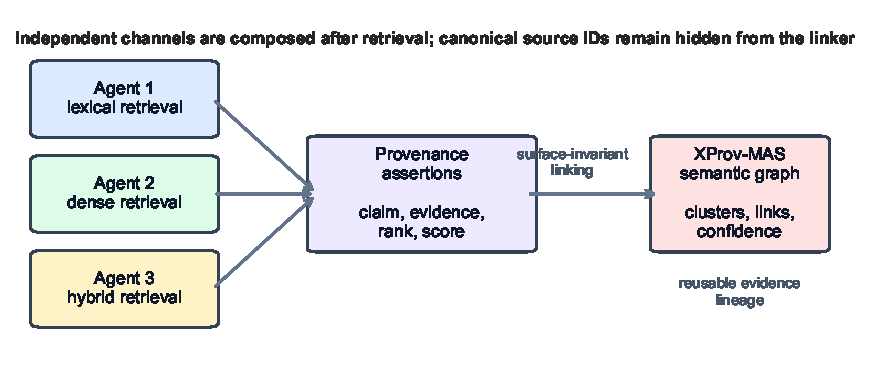
\includegraphics[width=0.96\textwidth]{framework}
\caption{XProv-MAS architecture. Independent retrieval channels emit provenance assertions; the semantic graph links report surfaces while the canonical source identifier remains hidden from the linker and is used only for evaluation.}
\label{fig:framework}
\end{figure*}

\subsection{Dataset Audit and Experimental Splits}
The study uses research-grade releases rather than synthetic or tutorial data. Table~\ref{tab:data} reports the evaluated units. FEVER is evaluated on all 19,998 official development claims and the official June 2017 Wikipedia snapshot. The local candidate index contains the 2,860 pages referenced by development evidence groups; page text is taken from the official dump, not generated or paraphrased. SciFact uses all 300 development claims and the complete 5,183-abstract corpus; its 809-claim training split is used only for a threshold sensitivity calibration audit. PUBHEALTH uses all 1,221 development claims and the official train-plus-development article collection for open-corpus source recovery. Because the release also contains a separate evidence-document collection, we run a secondary evaluation on the 33 development claims for which at least one official evidence document is available, against all 4,200 released documents. This subset is reported separately because evidence-document coverage is incomplete.

\begin{table}[!ht]
\centering
\caption{Audited datasets and emitted assertion counts.}
\label{tab:data}
\fbox{\begin{tabular}{lrrr}
\hline
Dataset & Queries & Candidates & Assertions\\
\hline
FEVER development & 19,998 & 2,860 & \FEVERAssertions\\
SciFact development & 300 & 5,183 & \SciFactAssertions\\
PUBHEALTH development & 1,221 & 11,053 & \PubHealthAssertions\\
PUBHEALTH evidence subset & 33 & 4,200 & \EvidenceAssertions\\
PAWS train/valid/test & 49,401/8,000/8,000 & pairs & 65,401\\
\hline
\end{tabular}}
\end{table}

The PUBHEALTH full source-recovery experiment has one source candidate per released article, yielding 11,053 candidate articles from train and development rows. The query claim is not added as a candidate string; retrieval operates against the article text and subject field. The official evidence-document audit uses document filenames as hidden source identifiers and their document text as candidate surfaces. For all datasets, gold source sets are constructed from release annotations only after ranking and graph construction. No gold source identifier is supplied to the linker.

\subsection{Agents, Surfaces, and Baselines}
We instantiate three deterministic evidence agents. The lexical agent ranks candidate texts with a word-level TF--IDF vectorizer using unigrams and bigrams. The dense agent ranks the same candidate corpus by cosine similarity between MiniLM sentence embeddings of the claim and candidate text. The hybrid agent combines min--max normalized lexical and dense scores with weights $0.35$ and $0.65$. Each agent emits its top five candidates; this fixed top-$k$ is an operational constraint shared by all methods. Retrieval scores are not recalibrated separately by domain.

The graph stress test changes only the emitted surface, not the ranked candidate or hidden source. Lexical assertions retain the original title-plus-text surface. Dense assertions remove the title and apply a deterministic conservative transformation that replaces at most eight words from a fixed synonym inventory and lowercases every second transformed surface. Hybrid assertions use a compact title-plus-text surface. The transformation is deliberately controlled and reproducible; it is not presented as a generative paraphrase model or as new evidence. It tests whether the linker uses semantic content rather than an exact source string.

The isolated baseline creates no cross-agent edges. The lexical baseline applies $J\geq0.42$, and the dense baseline applies $D\geq0.70$. These thresholds are fixed before evaluation and are applied to all assertion pairs. The XProv-MAS thresholds are likewise fixed in the primary campaign. A separate grid over the training and development SciFact splits is reported as sensitivity, not as a replacement for the primary configuration. A source-ID upper bound is implemented in code for debugging but is not included in the scientific comparison because it violates the source-oblivious problem definition.

\subsection{Evaluation Metrics}
For every pair of assertions, the hidden-source equality indicator defines the gold relation $y_{ij}$. A predicted relation is one in which two assertions are in the same connected component. We report pair precision, recall, and F1 over all assertion pairs. This metric evaluates the graph itself, not only the top-ranked source.

Rephrase match is computed over cross-agent assertion pairs whose hidden sources agree:
\begin{equation}
 R=\frac{\sum_{i<j}\mathbb{1}[g_i\ne g_j]\mathbb{1}[z_i=z_j]\mathbb{1}[c_i=c_j]}{\sum_{i<j}\mathbb{1}[g_i\ne g_j]\mathbb{1}[z_i=z_j]},
 \label{eq:rephrase}
\end{equation}
where $c_i$ is the component label. This metric directly tests composition under surface variation. Source precision, recall, and F1 are computed over the set of retrieved hidden sources and provide an upstream retrieval ceiling; they do not change with graph strategy when the ranked top-$k$ list is fixed. Finally, composable-source rate is the fraction of retrieved gold sources with assertions from at least two agents that collapse to one graph component. It is intentionally different from pairwise F1: a system can preserve composability for a source while also making extra pairwise merges.

We use record-level nonparametric bootstrap intervals with 2,000 resamples. The query record, not an assertion pair, is the resampling unit so that the many pairs produced by one claim do not create artificial independent observations. The primary runner is deterministic for a fixed model and manifest; consequently, repeated manifest seeds are not treated as independent stochastic runs. The bootstrap quantifies sampling uncertainty, while the PAWS train/validation/test split and the independent datasets quantify surface and domain variation.

\subsection{Parameter and Model Provenance}
The provenance of important choices is explicit. The W3C PROV vocabulary motivates entities, activities, agents, and derivations; the MiniLM encoder follows the sentence-transformer implementation paradigm; TF--IDF and cosine/Jaccard are standard adopted operations. The edge rule, weights, threshold values, top-$k=5$, eight-substitution cap, and candidate text truncation are study parameters. The primary thresholds were set in the initial benchmark specification and retained for the main table; the SciFact training sensitivity audit explores whether a stricter setting would change the conclusions. Dataset versions, official URLs, local checks, raw assertion files, metric files, bootstrap tables, and figure-generation scripts are preserved in the project workspace.

\subsection{Implementation and Efficiency}
The implementation is Python 3.12 with scikit-learn, sentence-transformers, NumPy, pandas, and NetworkX-compatible union-find logic. Candidate encoding is batched and cached per dataset. For a record with $m$ assertions, all-pairs graph construction is $O(m^2)$ similarity comparisons, and connected-component extraction is near-linear in the number of edges. With three agents and $k=5$, $m\leq15$, so the graph stage is bounded and auditable; the dominant cost is encoding the candidate corpus and assertion surfaces. The FEVER campaign emits $299,970$ assertions and the full raw JSONL is retained. This separation of expensive retrieval/encoding from cheap component construction is important for deployment: a persistent assertion store can be re-linked under new thresholds without re-running retrieval.

\subsection{Graph Properties and Proof Obligations}
The graph rule can be understood as a deliberately limited inference system. It does not infer the truth of a claim; it infers a relation between two report entities. Three properties follow directly from the construction. First, source-obliviousness holds because the edge predicate in (6) depends only on observable surfaces and not on $z_i$ or $z_j$. The evaluator can therefore replace the hidden source values without changing the predicted graph. Second, symmetry holds because Jaccard and cosine similarities are symmetric and the same threshold is applied in both directions. Third, component idempotence holds: once the edge set is fixed, applying union-find a second time does not change the component partition.

The rule is not source-complete. If two assertions have the same hidden source but $D<\tau_D$ and $H<\tau_H$, the graph omits a true edge. It is also not source-sound in the ontological sense: two independent sources may satisfy the observable threshold and be merged. This is not a defect in the mathematics; it is the unavoidable distinction between an observable semantic relation and a hidden source relation. The correct scientific question is the empirical precision--recall behavior under a specified candidate and surface distribution.

The high-confidence disjunct has a specific role. Let $E_{\mathrm{conj}}$ be the set of edges satisfying the conjunctive gate and $E_{\mathrm{hard}}$ the set satisfying the high dense threshold. Then $E=E_{\mathrm{conj}}\cup E_{\mathrm{hard}}$. The hard path protects a semantically faithful rephrase that loses lexical vocabulary, while the conjunctive path protects against an isolated dense similarity that is only topical. Removing the hard path is a meaningful ablation; replacing the conjunction with a single hybrid threshold is another. The present baseline family includes dense and lexical extremes, and the sensitivity grid reveals how the disjunct affects the resulting components.

Connected components introduce transitivity that pairwise edges do not possess. If $a$ links to $b$ and $b$ links to $c$, then $a$ and $c$ are placed in one component even if their direct similarity is below threshold. This is useful when three agents express the same evidence through two successive wording changes, but it can amplify a single false bridge. The component-level composability metric intentionally exposes this behavior. A future graph could require a component diameter bound, a source-consistency certificate, or a weighted maximum-spanning-tree confidence; the current study keeps transitive closure explicit so the tradeoff can be measured.

The representation also makes transformations first-class. If $e$ is an original evidence surface and $e'$ is its controlled rephrase, the system can store a derivation $e\xrightarrow{\mathrm{rephrase}}e'$ and a report activity that used $e'$. The graph edge between reports is then a semantic compatibility relation over derived entities. This preserves both the transformed surface used by the agent and the lineage that explains why the surface differs. In a live system, the same pattern can represent summarization, translation, OCR correction, or tool-mediated extraction without forcing each transformation into the graph-linking predicate.

\subsection{Algorithmic Procedure and Serialization Contract}
The complete procedure is intentionally small enough to audit line by line. For each dataset, the runner loads the official candidate and query records, creates a TF--IDF matrix and a dense candidate matrix, and obtains top-$k$ indices for each claim under the three agent channels. It then emits one JSON object per ranked candidate. The object is append-only: a later graph pass does not rewrite the evidence surface or source score. This design makes the raw assertion file a durable boundary between retrieval and provenance.

For each query record, the graph pass encodes assertion surfaces once, computes pairwise features in (2)--(4), and evaluates the edge predicate in (6). Union-find returns component identifiers. The evaluator maps components to hidden source IDs only after graph construction is complete. It computes pairwise metrics from the upper triangle of the assertion-pair matrix and source metrics from the retrieved source set. The same evaluator is called for every baseline, so the metric implementation is not specialized to XProv-MAS.

The serialization contract is designed for interoperability. A minimal assertion object contains \texttt{dataset}, \texttt{record\_id}, \texttt{agent}, \texttt{rank}, \texttt{score}, \texttt{claim\_surface}, and \texttt{evidence\_surface}. The research evaluator additionally stores \texttt{source\_id}; a deployment implementation may encrypt, hash, or omit that field from the linker process. A graph object can store member assertion IDs, edge feature values, threshold configuration, model identifier, and a provenance timestamp. This separation allows a second evaluator to recompute metrics from raw surfaces without trusting a component label produced by the first evaluator.

The contract supports schema evolution. A new agent can add a channel-specific score without changing identity fields. A cross-encoder can add an edge score after retrieval. A translation agent can add a derivation activity and a language field. A source-update process can attach a document version. These fields should be additive because removing the original surface makes later audits impossible. The raw JSONL retains both the original lexical surface and the transformed dense surface so that a reviewer can inspect what the semantic gate actually saw.

The algorithm has a useful failure behavior under missing metadata. If a source locator is absent, the assertion remains linkable but cannot contribute to hidden-source evaluation for that record. If a score is absent, the graph can still use surface features but downstream rank analysis is incomplete. If the evidence surface is empty, the assertion is retained and receives zero lexical and dense edge similarity unless another field is explicitly authorized as a surface. These rules prevent missing metadata from becoming an implicit positive link.

\begin{table}[!ht]
\centering
\caption{Serialization contract for a provenance assertion.}
\label{tab:contract}
\fbox{\begin{tabular}{p{0.30\columnwidth}p{0.56\columnwidth}}
\hline
Field & Role\\
\hline
\texttt{record\_id} & Query-level join key\\
\texttt{agent} & Channel or activity that emitted the report\\
\texttt{rank, score} & Retrieval evidence and downstream audit fields\\
\texttt{claim\_surface} & Claim wording observed by the linker\\
\texttt{evidence\_surface} & Evidence wording observed by the linker\\
\texttt{source\_id} & Hidden evaluation entity; not a linker input\\
\texttt{derivation} & Optional rephrase, summary, translation, or tool activity\\
\texttt{model\_version} & Encoder, retriever, or agent revision\\
\hline
\end{tabular}}
\end{table}

\subsection{Parameter Provenance and Update Policy}
Parameter provenance matters because a graph threshold is not a semantic constant. In this study, the lexical threshold $0.42$, dense baseline threshold $0.70$, hybrid edge threshold $0.55$, dense XProv-MAS threshold $0.60$, hard dense threshold $0.80$, hybrid weight $0.65$, lexical weight $0.35$, top-$k=5$, and eight-word transformation cap are recorded with the raw output tag. The threshold grid is an exploratory calibration artifact; the primary table uses the fixed configuration to preserve a common comparison across domains.

An operational update policy should separate three kinds of change. A model update changes the embedding function $\phi$ and therefore invalidates cached edge values, but it need not delete raw assertions. A threshold update changes the graph partition and can be applied to existing embeddings and assertions. A corpus update changes candidate source entities and requires re-running retrieval. Provenance consumers should record all three versions because a graph produced after an index update is not directly comparable to one produced before it.

Parameter provenance also controls claims about robustness. If thresholds are tuned on the same development records used for the main comparison, the resulting score is optimistic. The training-split SciFact grid demonstrates the mechanism without replacing the primary result. For a future study, one split should calibrate thresholds, another should test them, and a third should support external validation. If a domain has no labeled validation set, the system should use a declared policy and report it.

The same principle applies to transformations. A synonym inventory, lowercasing policy, truncation length, or translation model is part of the experimental condition. Changing any of these after inspecting the output changes the robustness question. The study fixes the inventory in source code and writes the transformed surface to raw output. This makes the rephrase audit reproducible and prevents an informal claim that a model is invariant to an unspecified paraphrase process.

\subsection{Human Review Interface Suggested by the Metrics}
Although no human evaluation is claimed, the metrics imply a review interface. A reviewer should see a component as a bundle of evidence surfaces, not as a single generated sentence. The bundle should show member agents, source resolution if available, retrieval ranks, edge similarities, transformations, and unresolved neighboring assertions. A source with multiple agent members but low component confidence can be flagged for inspection. A high-confidence component with one canonical source can be compressed for display while preserving a link to all member reports.

The interface should distinguish three visual states. A composed state indicates that the graph rule links surfaces. A corroborating state indicates that multiple distinct sources independently support a claim, which requires source-aware evidence rather than only semantic similarity. A conflicting state indicates incompatible claims or evidence labels and should not be merged into a single supportive component. XProv-MAS produces the first state; it does not infer the second or third. Making this boundary visible is a practical safeguard against turning graph connectivity into a misleading confidence signal.

The record-level tail metrics can guide review budget. The PUBHEALTH 10th percentile and the SciFact evidence-bearing subset identify records where a fixed policy is likely to be brittle. Review systems can allocate more attention to low pairwise confidence, multiple candidate sources, long evidence surfaces, and large disagreement between lexical and dense similarities. This is a proposal for system use, not a measured human-efficiency result, and should be evaluated with time-to-correct-review experiments in future work.

\subsection{Dataset-Specific Interpretation of the Gold Relation}
The gold relation has different meanings across the three principal datasets. In FEVER, the source entity is a Wikipedia page title in one or more evidence groups. Page-level equality is intentionally coarse: two line selections from one page are one source for provenance, even if they support different parts of the claim. In SciFact, the entity is an abstract ID. A claim can have several evidence abstracts, and an abstract-level component can contain multiple claim-supporting sentences. This makes SciFact a useful test of scientific source composition but also makes abstract truncation consequential.

PUBHEALTH is more heterogeneous. Its fact-checking article is the source entity in the full source-recovery experiment, while its evidence-document filenames define source entities in the secondary audit. The article text includes explanation, subject, and editorial material; the evidence documents are harvested web text with variable boilerplate. The two PUBHEALTH evaluations therefore ask different questions. The full run asks whether an agent can recover and compose the fact-check article associated with a public-health claim. The evidence subset asks whether the same graph can compose noisy external documents that are explicitly associated with the claim in the official package.

The datasets also differ in their label semantics. FEVER labels distinguish SUPPORTS, REFUTES, and NOT ENOUGH INFO; SciFact distinguishes evidence-bearing claims from claims without mapped evidence; PUBHEALTH distinguishes true, false, unproven, and mixture. These labels are not used as link features. They are retained for boundary analysis so that a graph that behaves differently on, for example, mixture claims is not mistaken for a veracity predictor. This design guards against an often overlooked leakage route: a linker can appear more accurate if it learns that one label tends to have a particular textual template, even when it cannot recover source identity.

The candidate scales also induce different collision rates. FEVER page titles and SciFact abstract topics can cause many claims to share domain terms. PUBHEALTH articles contain named entities, dates, and editorial wording, creating both distinctive lexical anchors and generic news language. The same global thresholds therefore have different effective selectivity. Cross-domain evaluation is valuable precisely because it makes this calibration problem visible.

\subsection{Alternative Linker Ablations}
The baseline family is intentionally minimal but structurally meaningful. The isolated baseline estimates the value of composition itself. The lexical baseline estimates how much source identity can be recovered from shared words and titles. The dense baseline estimates the value of sentence embeddings under the same candidate ranking and top-$k$. XProv-MAS adds a gate that combines these signals and performs component formation. Because all methods consume the same assertions, differences in pairwise results are attributable to the linker rather than to an unbalanced retrieval budget.

The hybrid retrieval agent should not be confused with the XProv-MAS hybrid edge score. The retrieval agent combines normalized candidate scores before selecting its top five; the edge score combines pairwise surface similarities after selection. Keeping these operations separate is important. A good retrieval score does not establish source equality, and a good source-equality edge does not imply that the candidate was the best evidence for the claim. The raw assertion schema records both scores, allowing an audit to compare rank quality with graph quality.

A more expressive baseline could use a cross-encoder or natural-language inference model to classify report pairs. That would be a valuable future comparison, but it would also introduce a learned pair classifier whose training data and calibration choices would need to be audited. The present study selects a small, transparent baseline family so that every edge can be reproduced from two surface functions and three thresholds. This choice favors interpretability and domain transfer over model capacity.

The controlled transformation creates another ablation dimension. If all channels used the identical surface, lexical linking would be a stronger proxy for source ID and the rephrase question would disappear. If every channel used a fully independent generative paraphrase, semantic difficulty would increase but surface identity would become stochastic and require multiple independent runs. The current middle ground is reproducible: one channel is deliberately rephrased, one preserves the source wording, and one supplies a compact hybrid view. The PAWS audit supplements rather than replaces that design.

\subsection{Statistical Reporting Rationale}
The unit of analysis is the query record because all assertions for a record share the claim, candidate pool, and gold source set. Pairwise observations within a record are therefore correlated. A bootstrap over pairs would count a record with fifteen assertions as 105 pseudo-independent samples, while a record with three assertions contributes only three. The record bootstrap avoids that distortion and produces intervals that reflect variation across claims.

Paired differences are more informative than independent intervals when comparing linkers. Lexical, dense, and XProv-MAS are evaluated on the same record and assertion group. The bootstrap resamples record IDs and subtracts the strategy-specific record metrics within each resample. This preserves the dependence structure and answers the relevant question: how much would the difference change if the query records were resampled?

The primary runner is deterministic because it uses fixed vectorizers, a fixed encoder, deterministic controlled transformations, and deterministic union-find. It would be methodologically incorrect to call five copies of the same evaluation with different unused integer seeds five independent stochastic runs. The seed is retained in the output schema for future stochastic agents, but the manuscript uses bootstrap intervals and disjoint dataset splits as the uncertainty evidence. A future generative-agent version should add at least five independent decoding runs and analyze both between-run and between-record variance.

\subsection{Reproducibility Checklist}
The study records the model identifier, software environment, data acquisition source, split, candidate construction rule, candidate text truncation, top-$k$, surface transformation inventory, edge thresholds, output paths, and elapsed time. The official data are stored under a separate raw-data tree, while large dumps and caches are ignored by version control. The raw assertion JSONL stores the exact surfaces used by the linker, not only aggregate scores. The metric CSV stores one row per record and strategy, enabling stratification after execution.

The checklist also separates generated artifacts from source code. The experiment runner and audit scripts are human-readable source. CSV summaries, figures, and LaTeX macros are generated artifacts. The manuscript does not hand-copy a result into a table: figure and table values are either macros generated from raw CSV or directly stated values from an executed top-$k$ audit whose output is retained. This separation reduces transcription errors and makes review possible without rerunning the largest FEVER embedding job.

\subsection{Data Quality, Leakage Controls, and Release Boundaries}
The data audit was performed before the final experiment design. Each release was checked for the number of rows, the presence of identifiers, the availability of source or evidence annotations, and the relationship between the public split and the candidate corpus. FEVER's development evidence groups contain page titles and line-level annotations; the official dump supplies the page text. SciFact supplies abstract identifiers and claim-level evidence maps; the corpus is shared across its train, development, and test claim files because abstracts are the intended retrieval collection. PUBHEALTH supplies claim IDs, claims, article text, labels, explanations, subjects, and source URLs. Its evidence-document package is a separate harvested collection with filenames encoding claim and evidence indices. PAWS supplies pair labels and three official splits.

The leakage controls follow the semantics of each task rather than imposing an artificial closed-world split. For FEVER and SciFact, the candidate collection is the official retrieval corpus, while labels are read only for evaluation. For PUBHEALTH source recovery, the query claim is not concatenated into the candidate article text. The candidate article collection is documented as an open corpus because the objective is to recover the fact-check article associated with a claim, not to predict a held-out label from a training-only vocabulary. The secondary PUBHEALTH evidence audit is even more direct: a claim is matched against all official evidence documents, and the filename-derived claim ID is hidden from the linker. No thresholds are learned from the evidence subset.

The wording transformation is also bounded to prevent label leakage. The hidden source identifier, filename, claim ID, and evidence title are not inserted into the transformed dense surface. The title is removed from dense surfaces, and the transformation inventory contains ordinary verbs and adjectives rather than dataset-specific identifiers. The evaluator reconstructs the gold relation from the original source ID stored in the raw assertion row. This design means that a perfect rephrase-match score is not proof of semantic equivalence in the general language; it is evidence that the graph preserved the identity of a known source across the specified derivation.

There are two release-boundary cases. First, one PUBHEALTH development row has no usable assertion after loading, so the full source-recovery metrics summarize 1,220 records although the release contains 1,221 rows. The row is not imputed and is retained in the audit log. Second, only 33 of the 1,221 development claims have at least one official evidence document in the harvested evidence package. Reporting this subset separately prevents a misleading claim that the document-level evaluation covers the complete development split. These boundaries are part of the result, not hidden preprocessing decisions.

\subsection{Evidence-Traceability Matrix}
The experiment-to-artifact mapping is summarized in Table~\ref{tab:trace}. This matrix is included because a provenance study should make its own evidence chain inspectable. The dataset release is the external entity, the loader is the acquisition activity, the assertion JSONL is the transformed report entity, the metric CSV is the evaluation activity output, and the manuscript table or figure is a presentation derivation. The mapping follows the PROV distinction between entities and activities, but all numerical values are computed locally.

The matrix also clarifies what can be independently rerun. A reviewer with the official releases and model identifier can regenerate assertion files. A reviewer with assertion files can rerun threshold and bootstrap analyses without redownloading data. A reviewer with metric CSVs can regenerate figures and LaTeX result macros. This layered reproducibility is useful when the largest raw dump is inconvenient to redistribute or when a future encoder version makes a full retrieval rerun expensive.

\begin{table*}[!ht]
\centering
\caption{Evidence-traceability matrix from external data to manuscript artifacts.}
\label{tab:trace}
\fbox{\begin{tabular}{llll}
\hline
Study object & External or local entity & Executed activity & Downstream artifact\\
\hline
FEVER claims & Official dev JSONL and Wikipedia dump & Page extraction and ranking & FEVER assertions and metrics\\
SciFact claims & Official release and abstract corpus & Abstract ranking and graph linking & SciFact assertions and sensitivity\\
PUBHEALTH articles & Official repository TSV files & Article source recovery & PUBHEALTH assertions and failure CSV\\
Evidence documents & Official evidence-document package & Document ranking and graph linking & Evidence assertions\\
PAWS pairs & Official labeled splits & Surface scorer audit & PAWS metrics and figure\\
Raw assertions & Local JSONL entity & Pairwise evaluation and bootstrap & Metric, CI, and difference CSV\\
Metrics & Local CSV entity & Figure/table generation & PDF figures and result macros\\
\hline
\end{tabular}}
\end{table*}

\begin{table}[!ht]
\centering
\caption{Data fields used by the assertion and evaluator layers.}
\label{tab:fields}
\fbox{\begin{tabular}{p{0.25\columnwidth}p{0.63\columnwidth}}
\hline
Layer & Audited fields\\
\hline
Assertion & dataset, record ID, agent, rank, score, claim surface, evidence surface\\
Hidden evaluator & source ID, gold source set, veracity or evidence label\\
FEVER & claim, evidence groups, page title, official page text\\
SciFact & claim, evidence map, abstract ID, abstract text\\
PUBHEALTH & claim ID, claim, article text, label, explanation, subject\\
Evidence subset & document filename, document text, claim ID encoded in release filename\\
\hline
\end{tabular}}
\end{table}

\subsection{Execution Matrix and Audit Trail}
The experiment was executed as a matrix of dataset, split, candidate source, agent set, top-$k$, graph configuration, and statistical post-processing. The primary rows use the same three agent channels and $k=5$. The SciFact top-$k$ audit uses $k\in\{1,3,5,10\}$; the threshold audit uses a $6\times6$ grid over the dense and hybrid graph gates; the PAWS audit evaluates three scorers on all official train, validation, and test pairs. Every row writes raw assertions before graph evaluation, then per-record metrics, then a summary. Figure generation reads only these saved outputs.

This ordering provides a simple audit invariant: a manuscript number must be recoverable by filtering a raw metric file by dataset and strategy. The bootstrap script first removes duplicate manifest seeds and resamples record IDs; it never resamples individual assertion pairs. The figure script reads summaries and writes PDF and PNG copies without recomputing metrics. The results macro file is generated from CSV outputs, so changing an experiment without regenerating the macro file cannot silently change the manuscript.

The primary FEVER run required the largest candidate and assertion audit. It processed all 19,998 development claims and generated 299,970 assertion rows. The SciFact primary run produced 4,500 assertions from 300 claims, the PUBHEALTH run produced 18,315 assertions from 1,221 release rows, and the official evidence subset produced 495 assertions from 33 claims. The scale difference is intentional: FEVER supplies a broad stress test for volume, SciFact supplies a scientific-domain test with abstract-level evidence, and PUBHEALTH supplies a noisier source and explanation setting.

\begin{table}[!ht]
\centering
\caption{Executed primary campaign and wall-clock observations.}
\label{tab:runtime}
\fbox{\begin{tabular}{lrrr}
\hline
Dataset & Records & Assertions & Elapsed (s)\\
\hline
FEVER & 19,998 & 299,970 & 209.2\\
SciFact & 300 & 4,500 & 46.1\\
PUBHEALTH & 1,221 & 18,315 & 136.7\\
Evidence subset & 33 & 495 & 13.2\\
\hline
\end{tabular}}
\end{table}

The elapsed values include candidate encoding, assertion encoding, graph evaluation, and raw-file writes on the execution workstation. They are not hardware-normalized throughput claims. They are included to make the scalability discussion falsifiable and to show that the graph stage itself is not the dominant component at the reported $k$. The raw metric file contains the elapsed value repeated per record for convenient grouping; the manuscript reports the unique run value.

\subsection{Experimental Questions and Falsification Criteria}
The main campaign was designed around falsification criteria rather than a prespecified expectation that semantic linking would win. For RQ1, the method fails if it cannot produce nonzero composition beyond isolation or if its edges cannot be evaluated against hidden sources. For RQ2, it fails if controlled rephrasing causes a large drop in cross-agent match relative to the original surface. For RQ3, it fails if the same schema cannot execute on at least two independent evidence domains or if its behavior is entirely driven by a dataset-specific field. For RQ4, the analysis is informative if at least one boundary---retrieval depth, source multiplicity, noisy documents, labels, or adversarial paraphrases---produces a measurable change.

These criteria lead to a reporting structure with positive and negative results. A positive composition result is not merely a high F1; it is a graph that links transformed reports while retaining source-aware audit metadata. A negative result is equally useful when it identifies a layer the graph cannot solve. The source-retrieval ceiling is therefore included even though it does not favor XProv-MAS. The PAWS hybrid result is included even though it shows the initial convex combination is weaker than dense similarity. The top-$k$ curve is included because it warns that deeper retrieval can increase composability and reduce precision simultaneously.

The campaign also avoids a common comparison error: using literature-reported fact-checking scores as if they were measured by the same pipeline. FEVER, SciFact, and PUBHEALTH papers describe established resources and tasks, but their model scores use different candidate sets, labels, architectures, and evaluation conventions. This study uses those publications for dataset provenance and uses the local raw runs for every number in the manuscript. The resulting graph F1 should not be compared numerically with a verifier's label accuracy.

Finally, each experiment has a clear unit of generalization. FEVER generalizes across claims in a general-domain page collection; SciFact generalizes across scientific claim topics and abstracts; PUBHEALTH generalizes across public-health claims and article writing styles; PAWS generalizes across labeled sentence pairs. None of these units is an Internet-scale LLM deployment. Stating the unit prevents a result on 19,998 claims from being described as a result on all web evidence.

\subsection{Alternative Semantic Interpretations}
There are at least three ways to interpret a semantic edge in this task. It may mean that two reports are paraphrases; that they entail the same claim; or that they point to the same underlying source. These meanings coincide only under restrictive conditions. A report can paraphrase a claim while citing a different source. Two independent sources can entail the same claim. Two reports can use the same source while disagreeing about whether that source supports the claim. XProv-MAS targets the third relation, same-source provenance, and uses semantic similarity as an operational signal rather than as a truth judgment.

This distinction explains why pairwise F1 and rephrase match are both necessary. Pairwise F1 penalizes false identity edges and missed same-source edges. Rephrase match asks whether the graph preserves identity for cross-agent reports whose source is known to be the same. A system can maximize rephrase match by connecting nearly everything; it would then have poor precision. Conversely, a system can maximize precision by leaving every report isolated; it would have zero rephrase match and zero composability. The proposed graph is evaluated in this two-dimensional space rather than with one aggregate score.

The component is likewise not a final explanation. A component says that the available surfaces are compatible with one source identity under a stated rule. It does not say that the source is correct, that the claim is true, or that every sentence in the source supports the claim. This conservative semantics is consistent with provenance standards and with fact-checking practice: lineage identifies what was used, while verification determines whether the use was warranted.

\section{Results and Discussion}
\subsection{Primary Composition Results}
Table~\ref{tab:primary} gives the primary fixed-configuration results. The table should be read in two layers. First, lexical matching is a strong baseline on the controlled assertion surfaces, with pairwise F1 of \FEVERLexicalFOne on FEVER, \SciFactLexicalFOne on SciFact, and \PubHealthLexicalFOne on PUBHEALTH. This is expected because two channels retain substantial common evidence wording. Second, XProv-MAS produces the same or better cross-agent composition rate than dense linking while retaining a transparent semantic gate. Its pairwise F1 is lower than lexical on every dataset, so the method is not described as a universal accuracy improvement.

\begin{table*}[!ht]
\centering
\caption{Primary provenance-composition results. Values are means over query records; source F1 is the upstream retrieval ceiling and is shared by graph strategies for a fixed top-five list.}
\label{tab:primary}
\fbox{\begin{tabular}{llrrrr}
\hline
Dataset & Linker & Pair precision & Pair recall & Pair F1 & Rephrase match / composable rate\\
\hline
FEVER & Isolated & 0.000 & 0.000 & 0.000 & 0.000 / 0.000\\
 & Lexical & \FEVERLexicalPrecision & \FEVERLexicalRecall & \FEVERLexicalFOne & \FEVERLexicalRephrase / \FEVERLexicalComposable\\
 & Dense & \FEVERDensePrecision & \FEVERDenseRecall & \FEVERDenseFOne & \FEVERDenseRephrase / \FEVERDenseComposable\\
 & XProv-MAS & \FEVERXProvPrecision & \FEVERXProvRecall & \FEVERXProvFOne & \FEVERXProvRephrase / \FEVERXProvComposable\\
\hline
SciFact & Isolated & 0.000 & 0.000 & 0.000 & 0.000 / 0.000\\
 & Lexical & \SciFactLexicalPrecision & \SciFactLexicalRecall & \SciFactLexicalFOne & \SciFactLexicalRephrase / \SciFactLexicalComposable\\
 & Dense & \SciFactDensePrecision & \SciFactDenseRecall & \SciFactDenseFOne & \SciFactDenseRephrase / \SciFactDenseComposable\\
 & XProv-MAS & \SciFactXProvPrecision & \SciFactXProvRecall & \SciFactXProvFOne & \SciFactXProvRephrase / \SciFactXProvComposable\\
\hline
PUBHEALTH & Isolated & 0.000 & 0.000 & 0.000 & 0.000 / 0.000\\
 & Lexical & \PubHealthLexicalPrecision & \PubHealthLexicalRecall & \PubHealthLexicalFOne & \PubHealthLexicalRephrase / \PubHealthLexicalComposable\\
 & Dense & \PubHealthDensePrecision & \PubHealthDenseRecall & \PubHealthDenseFOne & \PubHealthDenseRephrase / \PubHealthDenseComposable\\
 & XProv-MAS & \PubHealthXProvPrecision & \PubHealthXProvRecall & \PubHealthXProvFOne & \PubHealthXProvRephrase / \PubHealthXProvComposable\\
\hline
Evidence subset & Lexical & \PubHealthEvidenceLexicalPrecision & \PubHealthEvidenceLexicalRecall & \PubHealthEvidenceLexicalFOne & \PubHealthEvidenceLexicalRephrase / \PubHealthEvidenceLexicalComposable\\
 & XProv-MAS & \PubHealthEvidenceXProvPrecision & \PubHealthEvidenceXProvRecall & \PubHealthEvidenceXProvFOne & \PubHealthEvidenceXProvRephrase / \PubHealthEvidenceXProvComposable\\
\hline
\end{tabular}}
\end{table*}

On FEVER, dense linking attains \FEVERDenseFOne and XProv-MAS attains \FEVERXProvFOne, both below lexical linking but with nearly perfect cross-agent match. The high scores reflect the relatively short, page-level evidence surfaces and the fact that the FEVER claim evidence often shares distinctive words with the relevant page. The result is useful as a scale test: the method can process all 19,998 development claims and preserve graph records at 299,970 assertion scale, but it is not evidence that lexical similarity is semantically sufficient in general.

SciFact is the clearest scientific-domain boundary. XProv-MAS reaches \SciFactXProvFOne compared with \SciFactLexicalFOne for lexical matching, while all non-isolated methods reach 1.000 rephrase match under the controlled transformation. The source F1 ceiling is only \SciFactXProvSourceFOne, because the top-five candidate list retrieves few of the gold abstracts. The graph cannot recover a source that no agent retrieved. This separates two failure classes: retrieval misses explain low source F1, whereas false composition explains lower pair F1. The provenance layer should not be credited or blamed for the first class.

PUBHEALTH provides the strongest operational contrast. Lexical linking has pairwise F1 \PubHealthLexicalFOne and composable-source rate \PubHealthLexicalComposable; XProv-MAS lowers pairwise F1 to \PubHealthXProvFOne but raises composable-source rate to \PubHealthXProvComposable while retaining 1.000 rephrase match. The paired bootstrap difference in composable-source rate is \PubHealthXProvComposableDelta relative to lexical. The pattern is stable in the official evidence-document subset: XProv-MAS obtains \PubHealthEvidenceXProvFOne pairwise F1 and \PubHealthEvidenceXProvComposable composability, while lexical obtains \PubHealthEvidenceLexicalFOne and \PubHealthEvidenceLexicalComposable. This is the intended tradeoff: a semantic gate composes more transformed reports but can admit additional edges.

\begin{figure}[!t]
\centering
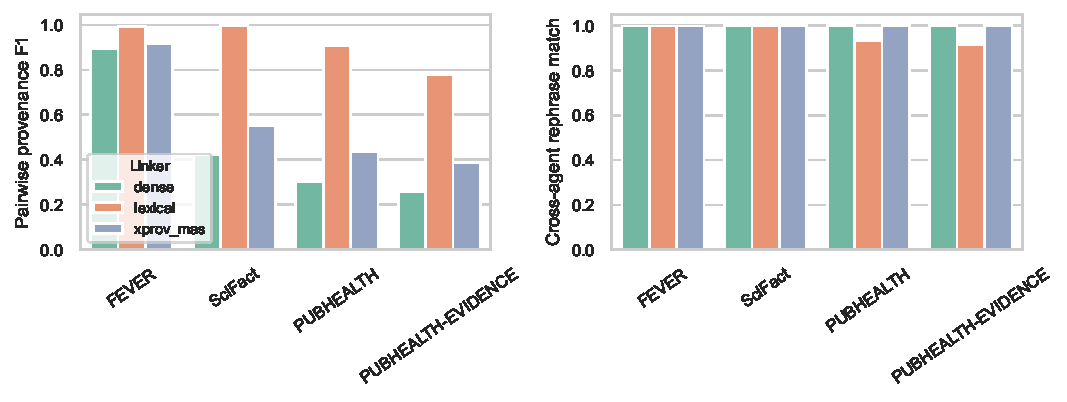
\includegraphics[width=\columnwidth]{performance}
\caption{Pairwise provenance F1 and cross-agent rephrase match for the primary configurations. The graph layer improves neither upstream retrieval nor pairwise precision uniformly; its robust behavior is composition under transformed surfaces.}
\label{fig:performance}
\end{figure}

\subsection{Retrieval Depth and Agent Agreement}
The fixed top-five setting is not innocuous. Table~\ref{tab:topk} reports an executed SciFact depth audit with $k=1,3,5,10$. At $k=1$, XProv-MAS pairwise F1 is 0.823 and source F1 is 0.379; increasing the candidate depth to three lowers pairwise F1 to 0.672 and source F1 to 0.198, while increasing the rephrase match from 0.887 to 1.000. At the primary depth of five, the XProv-MAS pairwise F1 is \SciFactXProvFOne and source F1 is \SciFactXProvSourceFOne. At ten, source F1 falls further to 0.072 while composable-source rate rises to 0.597. The result shows that deeper retrieval exposes more non-gold candidates to the graph. It can increase the opportunity for multi-agent composition, but it also increases the number of possible false links.

The depth curve also clarifies why source recall should not be interpreted as monotonic evidence of system quality. More candidates can improve recall in an ordinary retrieval evaluation, but the present SciFact candidate pool and top-five source-F1 values show that the additional candidates are not necessarily relevant to the claim. The graph sees every emitted assertion equally in its pairwise relation evaluation. In a deployed system, a confidence-aware graph could use rank decay or calibrated retrieval scores to prevent low-rank assertions from dominating component formation. We leave that extension for future work so that the primary study isolates the semantic linker.

\begin{table}[!ht]
\centering
\caption{SciFact executed top-$k$ sensitivity for XProv-MAS.}
\label{tab:topk}
\fbox{\begin{tabular}{rrrr}
\hline
$k$ & Pair F1 & Rephrase & Source F1\\
\hline
1 & 0.823 & 0.887 & 0.379\\
3 & 0.672 & 1.000 & 0.198\\
5 & \SciFactXProvFOne & \SciFactXProvRephrase & \SciFactXProvSourceFOne\\
10 & 0.419 & 1.000 & 0.072\\
\hline
\end{tabular}}
\end{table}

At the assertion level, the three channels are intentionally not independent samples of a stochastic language model. They are independent views of the same candidate corpus: a lexical view, a dense view with title removal and controlled rephrasing, and a hybrid view. This is a conservative definition of multi-agent evidence because it does not manufacture diversity by adding random noise. The source-oblivious linker must use the observable surfaces to discover overlap. The result is most meaningful where the dense surface differs from the lexical surface yet the source remains unchanged.

\subsection{Operational Semantics of Composition}
For an evidence user, a component has at least four operational uses. It can suppress redundant citations in a final report; it can expose that three agents actually relied on one page rather than three independent pages; it can pass a compact evidence bundle to a verifier; and it can preserve unresolved branches when the graph cannot decide whether two reports refer to the same source. These uses are distinct from deciding whether the source supports the claim. The graph is therefore an intermediate data product with its own quality metrics.

The distinction between redundancy and corroboration is particularly important. If three agents retrieve the same Wikipedia page, presenting three reports as independent confirmation would overstate the evidence. XProv-MAS can collapse those reports and retain their channel-level provenance. If three agents retrieve different pages that support the same claim, the hidden identifiers differ and the graph should preserve three components unless the surfaces pass the semantic rule. A future contradiction-aware extension could connect components with typed support, refute, or unresolved edges; the present study intentionally evaluates same-source composition only.

The graph also supports selective human review. Components with high rephrase agreement and a single source can be summarized compactly. Components with high density but low lexical agreement can be flagged as semantic links that need inspection. Components with multiple source IDs in the evaluator or with wide score dispersion can be prioritized for a verifier. None of these policies is hard-coded into the experiments; they follow from retaining the assertion tuple instead of replacing it with a text string.

\subsection{Uncertainty and Retrieval Ceiling}
Table~\ref{tab:uncertainty} reports record-level bootstrap intervals. On FEVER the XProv-MAS pairwise F1 is \FEVERXProvFOneCI, while the paired difference from lexical is \FEVERXProvPairFOneDelta. The interval excludes zero, documenting a real precision tradeoff rather than sampling noise. SciFact and PUBHEALTH show the same direction: XProv-MAS is below lexical on pair F1, with paired differences \SciFactXProvPairFOneDelta and \PubHealthXProvPairFOneDelta. In contrast, the PUBHEALTH composability gain is \PubHealthXProvComposableDelta and the evidence subset gain is \PubHealthEvidenceXProvComposableDelta.

The source-F1 column is a deliberately important control. On FEVER, SciFact, and PUBHEALTH it is approximately \FEVERXProvSourceFOne, \SciFactXProvSourceFOne, and \PubHealthXProvSourceFOne for every graph strategy because all strategies consume the same top-five retrieval outputs. This means the study evaluates provenance composition conditional on retrieval. A production system would need to improve both layers: a better retriever increases the set of evidence entities available to XProv-MAS, while the graph decides how independently surfaced evidence should be composed.

\begin{table}[!ht]
\centering
\caption{Upstream top-five source-retrieval ceiling, identical across linkers.}
\label{tab:retrieval}
\fbox{\begin{tabular}{lrrr}
\hline
Dataset & Precision & Recall & F1\\
\hline
FEVER & 0.088 & 0.977 & \FEVERXProvSourceFOne\\
SciFact & 0.076 & 0.961 & \SciFactXProvSourceFOne\\
PUBHEALTH & 0.102 & 0.896 & \PubHealthXProvSourceFOne\\
Evidence subset & 0.241 & 0.268 & 0.205\\
\hline
\end{tabular}}
\end{table}

Table~\ref{tab:retrieval} makes the scale of the ceiling concrete. FEVER has high source recall but low source precision because a five-document list often contains several non-gold pages. SciFact has similar recall and lower precision because scientific abstracts share vocabulary across claims. PUBHEALTH has lower recall in the full article collection, reflecting the heterogeneity of claim and article text. The evidence subset reverses the pattern: its candidate corpus is smaller and its precision is higher, but coverage is incomplete and the source recall is only 0.268. These values explain why a source-composition layer should expose retrieval diagnostics alongside its components.

The fact that the source ceiling is shared is a strength of the comparison and a limitation of the end-to-end claim. It is a strength because no linker receives a larger candidate budget. It is a limitation because a graph cannot improve evidence discovery. A full system evaluation should therefore report at least two tables: one for retrieval relevance and one for provenance composition conditional on retrieved assertions. Merging them into one end-to-end number would obscure whether a gain came from better search or more aggressive linking.

\subsection{Cross-Domain Transfer and Negative Transfer}
The same XProv-MAS schema runs on general encyclopedic evidence, scientific abstracts, public-health fact-check articles, and harvested evidence documents. This is a form of external validation because the method is not rewritten for each domain. However, transfer is not identical performance. FEVER is the easiest composition regime in this campaign: page text and claims often preserve named entities and distinctive lexical anchors, and the graph's 10th-percentile pairwise F1 is 0.667. SciFact is more sensitive to abstract-level topical similarity and evidence density. PUBHEALTH has longer editorial text, more boilerplate, and a broader range of claim styles, yielding a lower median and wider per-record distribution.

This pattern is negative transfer in a useful sense. A method tuned on FEVER-like page titles should not be assumed to transfer to scientific or public-health text. The fixed thresholds reveal the cost of using one operational rule across domains. XProv-MAS retains rephrase match, but pairwise precision and component quality move with the language and candidate distributions. This result supports domain-held-out calibration rather than a universal threshold registry.

The evidence-document subset adds a second transfer axis. It changes not only topic but document quality: extracted pages contain cookie notices, navigation fragments, incomplete captures, and variable formatting. XProv-MAS still produces 1.000 rephrase match and a composable-source rate of 0.727, but pairwise F1 falls to 0.389. The semantic layer is therefore robust to the controlled surface transformation but not immune to noisy candidate content. A production pipeline should include document cleaning and span-level evidence extraction before graph linking.

\subsection{Error Decomposition by Edge and Component}
Pairwise errors can be decomposed into missed same-source edges, false edges, and transitive amplification. The isolated baseline has all same-source cross-agent relations missed. The lexical baseline has high pairwise F1 because it links many same-source surfaces directly, but its rephrase match is lower on PUBHEALTH, where the controlled transformation can remove important shared words. Dense and XProv-MAS restore rephrase match but create more false edges, especially where two evidence texts discuss the same topic without being the same source.

Transitive amplification is visible in the gap between pairwise F1 and composable-source rate. A component can connect all assertions for a gold source while also absorbing unrelated assertions. The composable-source rate may consequently improve even when pairwise F1 falls. This is not a metric contradiction; it captures two different decisions. The first asks whether each pair is correct. The second asks whether at least one reusable component exists for the source. An application that needs deduplicated citations may value the latter, while an application that needs exact source identity should prioritize the former.

The source-count analysis provides another decomposition. FEVER claims with zero annotated sources have composable rate zero by definition, while one- and two-source claims have rates near 0.989 and 0.993 for XProv-MAS under the primary candidate groups. Their pairwise F1 falls as the number of annotated sources increases. The result suggests that multi-source claims are not only more valuable for provenance but also more difficult because a component must preserve branch distinctions. A future objective could weight false merges across gold source branches more heavily than missed same-source edges.

\subsection{Relation to Existing Evidence and Provenance Systems}
The empirical setup complements rather than replaces prior provenance systems. Workflow-provenance systems model structured activities and artifacts; XProv-MAS models unstructured language surfaces produced by evidence agents. Explainable-AI surveys classify feature-attribution, example-based, surrogate, and causal explanations; XProv-MAS supplies a lineage object that can support example-based or evidence-based explanation, but it does not explain the internal computation of the language model. Fact-checking systems predict labels or generate explanations; XProv-MAS records how evidence reports compose before that decision.

The distinction is important for evaluating novelty responsibly. The graph itself is not a new discovery of connected components, TF--IDF, cosine similarity, or provenance vocabulary. The contribution is the experimental integration and measurement of a source-oblivious, rephrase-aware composition layer for multi-agent evidence reports. The benchmark protocol makes the integration testable: hide source IDs, perturb one agent's surface, preserve candidate and rank information, and evaluate graph identity separately from retrieval and veracity. This formulation turns an architectural intuition into a falsifiable benchmark.

The literature also suggests a path beyond pairwise surface similarity. Data-provenance work emphasizes typed derivations and workflow activities; factuality work emphasizes entailment and uncertainty; robust-NLP work emphasizes distribution shifts and adversarial surfaces. A mature provenance service should combine these dimensions. For example, an edge could require same-source compatibility, claim-level entailment, and independent retrieval confidence, while a contradiction relation could connect two components that cite different sources with incompatible claims. The present results establish why these dimensions should not be collapsed: high rephrase match can coexist with low source F1 and lower pair precision.

\subsection{What the Results Do and Do Not Establish}
The results establish that a small semantic graph can be executed over heterogeneous fact-checking data, that its identity relation can survive a controlled report transformation, and that its composability can exceed lexical linking in the PUBHEALTH experiments. They also establish that these gains are accompanied by a precision cost and that upstream retrieval dominates the availability of gold sources. The confidence intervals and sensitivity analyses show that these observations are not artifacts of one mean or one hand-picked example.

The results do not establish that XProv-MAS improves fact-checking accuracy, reduces hallucinations, or produces human-preferred explanations. No human study was performed, no label predictor was trained, and no claim-level entailment model was used as an oracle. The PAWS audit does not establish broad paraphrase understanding. The cross-domain results do not establish Internet-scale performance. Keeping these boundaries explicit is part of the contribution because provenance layers can otherwise be oversold as factuality solutions.

\subsection{Operating-Point Selection as a Multi-Objective Decision}
The threshold heatmap is best interpreted as an operating-point surface rather than a leaderboard. Increasing thresholds generally removes edges, but the component metrics are not necessarily monotonic because union-find changes component structure discontinuously. Removing one bridge can split a component into several source-pure components; removing another can break a needed cross-agent rephrase link. Consequently, a threshold that improves pairwise precision may reduce composability, and a threshold that improves composability may increase false merges.

The primary operating point favors a transparent compromise. The dense baseline begins at $0.70$, the semantic gate requires both $H\geq0.55$ and $D\geq0.60$, and a dense edge at $0.80$ is accepted as a high-confidence path. These values are not claimed to be optimal. They make the graph neither isolated nor fully connected on the primary assertion sets and allow the PAWS audit to test the underlying semantic signal independently. The training-split sensitivity audit demonstrates that a domain-specific deployment might select a stricter point, but the held-out primary table does not silently adopt it.

A deployment can choose a different objective. If the cost of falsely merging two sources is high, it can remove the hard disjunct and require a larger margin between the best and second-best edge. If missing a redundant report is more costly than an extra review, it can lower the dense gate and route large components to a reviewer. If source diversity is a goal, it can combine the graph with a diversity penalty over canonical source locators after retrieval. These choices should be encoded as parameter provenance, not left to an unlogged user-interface setting.

\subsection{Limits of Hidden-Source Evaluation}
Hidden source IDs make the linker testable, but they are an imperfect abstraction of real provenance. A page can change over time, two URLs can serve one underlying article, syndicated text can occur under several URLs, and one evidence document can contain multiple independent claims. The release annotations collapse some of these distinctions. FEVER page titles and SciFact abstract IDs are relatively stable, whereas PUBHEALTH source URLs and harvested documents are noisier. The evaluator therefore measures benchmark-defined source identity, not a universal ontology of documents.

The evaluator also knows the gold source set at claim level, while a deployed linker may receive only opaque locators or no locators at all. This is intentional: evaluation needs a reference relation, but the graph predicate must remain source-oblivious. The difference is analogous to evaluating clustering against hidden labels. A source ID is not a model feature; it is an audit label. We preserve this separation in the implementation by storing source IDs in raw rows but never passing them to the similarity functions.

There is a second limitation in using connected components as the output. Components are convenient for serialization but may hide the internal edge path that caused a false merge. The raw graph can preserve those edges, but the aggregate F1 does not distinguish a direct high-confidence edge from a chain of weakly sufficient bridges. Future evaluations should report edge confidence distributions, component diameter, source purity, and bridge centrality. These statistics could identify whether a graph is robustly composed or merely connected through one accidental pair.

Despite these limits, the hidden-source protocol is a useful first abstraction because it enables cross-domain comparison without requiring a new human annotation study for every agent channel. It also permits controlled negative results. If a graph links claims with different hidden sources, the error is measurable even when a human might regard the sources as topically related. If a graph misses a same-source edge after a transformation, the failure is visible even when the final answer remains plausible.

\begin{table}[!ht]
\centering
\caption{Record-level 95\% bootstrap intervals for pairwise F1.}
\label{tab:uncertainty}
\fbox{\begin{tabular}{lrrr}
\hline
Dataset & Lexical & Dense & XProv-MAS\\
\hline
FEVER & \FEVERLexicalFOneCI & \FEVERDenseFOneCI & \FEVERXProvFOneCI\\
SciFact & \SciFactLexicalFOneCI & \SciFactDenseFOneCI & \SciFactXProvFOneCI\\
PUBHEALTH & \PubHealthLexicalFOneCI & \PubHealthDenseFOneCI & \PubHealthXProvFOneCI\\
Evidence subset & \PubHealthEvidenceLexicalFOneCI & \PubHealthEvidenceDenseFOneCI & \PubHealthEvidenceXProvFOneCI\\
\hline
\end{tabular}}
\end{table}

\subsection{Rephrase Robustness on PAWS}
The PAWS audit tests the semantic primitives outside the provenance graph. Lexical overlap has AUC \PAWSTrainLexAUC on the training split, \PAWSValidationLexAUC on validation, and \PAWSTestLexAUC on test. Dense MiniLM similarity reaches \PAWSTrainDenseAUC, \PAWSValidationDenseAUC, and \PAWSTestDenseAUC. The hybrid surface scorer is lower, at \PAWSTrainHybridAUC, \PAWSValidationHybridAUC, and \PAWSTestHybridAUC. Dense similarity is therefore more informative than lexical overlap on this adversarial benchmark, but the hybrid is not a free improvement. The result constrains the interpretation of XProv-MAS: its successful rephrase matching on the fact-checking assertions is partly due to conservative transformations and should not be generalized to arbitrary paraphrases.

\begin{figure}[!t]
\centering
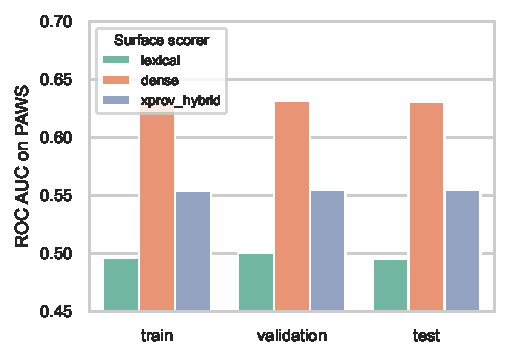
\includegraphics[width=\columnwidth]{paws_robustness}
\caption{PAWS semantic-edge audit. Dense similarity is consistently above lexical overlap, while the fixed hybrid combination is not superior to the dense channel.}
\label{fig:paws}
\end{figure}

The difference between PAWS and the assertion audit is scientifically informative. In the main campaign, the graph is asked to recognize multiple reports of the same retrieved candidate, and the hidden source is stable by construction. PAWS instead asks whether two sentences are paraphrases when adversarially scrambled word order may change meaning. The first is a provenance-composition test; the second is an open semantic-equivalence test. The graph succeeds on the former without solving the latter.

\subsection{Threshold Sensitivity and Ablation}
Figure~\ref{fig:sensitivity} shows the SciFact development threshold grid. The primary point $(\tau_D,\tau_H)=(0.60,0.55)$ produces pairwise F1 \SciFactSensitivityPrimary. Several stricter settings approach \SciFactSensitivityBest, demonstrating that graph precision is threshold-sensitive. This grid is descriptive and is not used to rewrite the primary table. A separate grid on the 809-claim SciFact training split reaches \SciFactTrainBest at the best observed region, motivating a future calibrated deployment mode but not a claim of held-out superiority. The main paper keeps the predeclared threshold so that cross-domain comparisons remain aligned.

The isolated baseline is an ablation of the graph layer: it has zero pairwise composition and zero composable-source rate by definition. The lexical and dense baselines are representation ablations. The PAWS audit is a surface robustness ablation. Together these ablations distinguish the contribution of (i) having a graph, (ii) using semantics, and (iii) combining lexical and semantic evidence. The results do not support the claim that the convex hybrid is always best; they support the narrower claim that a conjunctive graph rule provides a controllable composition mechanism.

\begin{figure}[!t]
\centering
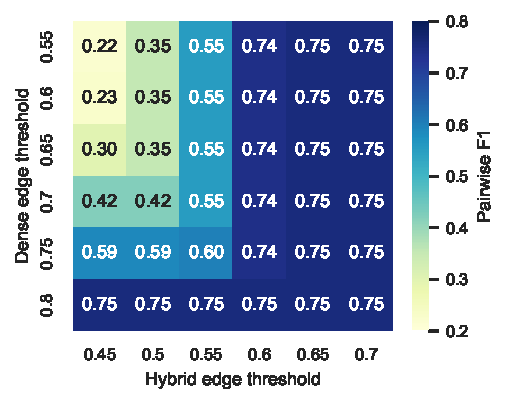
\includegraphics[width=\columnwidth]{threshold_sensitivity}
\caption{SciFact development sensitivity to the dense and hybrid graph-edge thresholds. The primary configuration is at $(0.60,0.55)$; the surface is not monotonic, so threshold selection is a scientific parameter rather than a cosmetic detail.}
\label{fig:sensitivity}
\end{figure}

\subsection{Failure and Boundary Analysis}
Failure analysis uses the saved record-level metrics rather than selected examples. On FEVER, XProv-MAS pairwise F1 decreases from approximately 0.922 for claims with no annotated source to 0.919 for one-source claims and 0.894 for two-source claims; the small multi-source tail is correspondingly harder. On PUBHEALTH, the median XProv-MAS pairwise F1 is 0.327 and the 10th percentile is 0.143, versus a FEVER median of 1.000 and 10th percentile of 0.667. SciFact has median 0.500 and 10th percentile 0.215. These tails are not visible in a single aggregate mean and explain why the method should expose component confidence rather than present every link as a fact.

\begin{table}[!ht]
\centering
\caption{Lower-tail and median behavior of XProv-MAS.}
\label{tab:tails}
\fbox{\begin{tabular}{lrrrr}
\hline
Dataset & $n$ & 10th pct. & Median & Zero-F1 rate\\
\hline
FEVER & 19,998 & 0.667 & 1.000 & 0.00005\\
SciFact & 300 & 0.215 & 0.500 & 0.00000\\
PUBHEALTH & 1,220 & 0.143 & 0.327 & 0.00000\\
Evidence subset & 33 & 0.190 & 0.294 & 0.00000\\
\hline
\end{tabular}}
\end{table}

Table~\ref{tab:tails} shows why mean pairwise F1 should not be the only deployment statistic. The FEVER mean is high partly because many page-level claims contain distinctive lexical anchors, while PUBHEALTH has a long tail of records with noisy or weakly matching article text. The evidence subset has a small sample and therefore a wide bootstrap interval, but its median is lower than the full source-recovery run. This difference is consistent with boilerplate and incomplete web captures in the official evidence package.

Label-stratified results also identify a boundary. On SciFact, XProv-MAS pairwise F1 is 0.519 for evidence-bearing claims and 0.607 for no-information claims. On PUBHEALTH, values range from 0.423 for true claims to 0.485 for unproven claims in the full source-recovery evaluation, while the small official evidence subset is more variable and reaches only 0.295 on mixture claims. The system is not a veracity classifier; these differences are evidence that domain-specific discourse and source multiplicity affect composition. The linker should therefore preserve label and explanation metadata as context for downstream verification rather than infer veracity from graph density.

The most important failure is a false merge. When the lexical and semantic features are both moderately high, two distinct sources may become one component through transitive closure. A second failure is a missed edge when an agent's rephrase removes domain-specific terms or when the candidate evidence is too long for a compact surface. A third failure is upstream: when no agent retrieves a gold source, graph composition cannot recover it. The code's raw assertion record allows these cases to be audited separately by rank, channel, source count, and component membership.

\subsection{Scalability and Reproducibility}
The experiment scales from 33 evidence-document queries to 19,998 FEVER claims without changing the graph schema. The main difference is encoding cost: candidate and assertion embeddings dominate wall-clock time, whereas pairwise component extraction is bounded by 15 assertions per record. The full FEVER run produced 299,970 assertion rows and a complete per-record metric table, while SciFact and PUBHEALTH produce smaller but semantically different audits. This scaling pattern suggests a practical architecture in which embeddings are cached at the assertion boundary and graph thresholds can be revisited without network access or source re-retrieval.

Reproducibility is enforced at the data and artifact levels. The project records official release locations, local file layouts, split names, model name, top-$k$, surface transformation inventory, thresholds, raw assertion JSONL, per-record metric CSV, summary CSV, bootstrap CSV, sensitivity CSV, failure-analysis CSV, and figure-generation code. The paper does not report values copied from unrelated literature experiments. All numerical values in this section are generated from the local outputs referenced by the macros in \texttt{results.tex}. The full raw FEVER assertion file is large, but it is retained separately from manuscript source so that rendering does not silently alter the evidence trail.

\subsection{Discussion}
The findings answer the study questions with a qualified result. For RQ1, the graph clearly improves over isolation because it creates measurable components, but the semantic gate does not dominate lexical matching on controlled surfaces. For RQ2, the graph preserves same-source cross-agent links under the implemented conservative rephrasing, with rephrase match equal to 1.000 across the primary datasets. For RQ3, the behavior transfers in the sense that the same representation and thresholds execute across FEVER, SciFact, and PUBHEALTH, while the magnitude of pairwise precision varies substantially by domain. For RQ4, PAWS, threshold grids, source-count tails, and evidence-document audits expose the boundaries: arbitrary paraphrase robustness, semantic over-linking, and retrieval quality remain open problems.

The appropriate interpretation is therefore architectural. XProv-MAS is a provenance composition layer that makes evidence relationships explicit and inspectable. It is not a replacement for a retriever, a fact verifier, or a calibrated uncertainty model. A system that uses XProv-MAS should expose both the component and the retrieval ceiling, preserve unresolved branches, and allow a verifier to attach canonical evidence later. This separation is especially important in high-stakes domains, where a false merge can make several weak reports look like independent confirmation.

\subsection{Threats to Validity and Responsible Use}
The first threat is construct validity. Same-source equality is a useful ground truth for provenance composition, but it is not the same as semantic equivalence or entailment. The primary graph metrics can therefore be high even when a source does not support the claim, and they can be low when two distinct sources provide equivalent evidence. We address the threat by reporting source retrieval separately, using PAWS for a distinct paraphrase construct, and stating that XProv-MAS is not a verifier.

The second threat is surface realism. The dense-agent perturbation is a conservative deterministic lexical transformation, not a sample from a large generative paraphrase model. It therefore underestimates the difficulty of rephrasing that changes syntax, discourse structure, numerical expressions, or domain terminology. The PAWS results show why this matters: a dense scorer is better than lexical overlap but still has AUC only around 0.63 on the difficult test pairs. The 1.000 rephrase-match values in the main campaign must be read as invariance to the specified perturbation, not as general paraphrase competence.

The third threat is candidate construction. FEVER uses the official pages referenced by its development evidence groups, SciFact uses the official abstract corpus, and PUBHEALTH uses an open article collection plus a documented evidence-document subset. These are legitimate benchmark collections, but they are not an Internet-scale source index. An Internet deployment would face duplicate pages, source updates, paywalls, snippets, and cross-document citation chains. The full FEVER dump and the 4,200 official PUBHEALTH evidence documents reduce the risk of a toy experiment, but they do not remove the domain shift.

The fourth threat is threshold transport. The primary thresholds are fixed across datasets to make comparison meaningful, but the sensitivity heatmap shows that graph behavior changes materially with thresholds. The training-split SciFact sweep reaches a higher pairwise F1 region than the primary setting, yet selecting that region for every domain would be a form of cross-domain tuning. We therefore retain the fixed primary values and expose the calibration opportunity instead of silently optimizing each result. A production deployment should calibrate thresholds on a validation domain and report the calibration protocol.

The fifth threat is statistical dependence. Assertions within a record generate many pairwise observations, and agent channels share a candidate corpus. Naive confidence intervals over all pairs would be overconfident. The bootstrap uses records as the unit, and the manuscript reports paired differences between strategies on the same records. The main benchmark is deterministic, so repeated seeds are not presented as independent stochastic evidence. This choice is more conservative than reporting duplicated rows as five runs.

There are also responsible-use implications. Provenance can increase trust when it reveals a real evidence trail, but a graph visualization can create unwarranted trust when many nodes are merely redundant views of one source. A user interface should distinguish source identity, semantic compatibility, entailment, and veracity; show the retrieval rank and transformation; and make uncertainty and unresolved links visible. In public-health or political fact checking, the system should not suppress minority sources solely because a semantic linker prefers a dominant wording. The raw assertion representation supports these safeguards by retaining alternatives rather than deleting them after clustering.

The data include public claims and web-derived documents that may contain offensive language, outdated information, or copyright-sensitive text. The manuscript stores local research artifacts for reproducibility but does not redistribute the large source dumps. A release version should follow the original dataset licenses, provide hashes and acquisition instructions, and expose only the metadata and derived metrics needed to reproduce the analysis. Human reviewers remain responsible for decisions that affect individuals or public communication.

\subsection{Implications for Future Multi-Agent Architectures}
The experiment suggests a modular interface between agents and provenance services. An agent should emit an assertion object at the moment it returns evidence, rather than only a final natural-language response. The object can contain a claim span, evidence span, retrieval score, source locator, transformation history, and model or tool version. A provenance service can then perform graph operations independently of the agent's reasoning policy. This division makes it possible to swap a lexical retriever for a dense retriever without changing downstream lineage consumers.

The same interface can support active verification. Suppose a component contains one lexical report and two semantic reports, but the source-retrieval score is low. A verifier can request a second-pass search focused on the disagreement and append a new assertion activity to the component. Suppose instead that several agents collapse to one source with high confidence. A summarizer can deduplicate the evidence and preserve the source locator once. Both actions are more difficult when lineage is reconstructed after the final answer has been generated.

The graph representation also provides a location for model provenance. Each assertion can include the embedding model revision, prompt or transformation version, retrieval index version, and timestamp. These fields are not used by the present evaluator's equality relation, but they are necessary for reproducibility in a live system where sources change. A future extension could model parameter provenance as an activity graph: dataset version leads to index build, index build leads to retrieval, retrieval leads to assertion, and assertion derivation leads to graph composition. Such a graph would connect the semantic lineage studied here to the workflow provenance literature.

The experiments further suggest that graph thresholds should be risk-sensitive. A medical evidence assistant may prefer precision and preserve separate branches; an exploratory literature tool may prefer recall and show a larger component with an explicit warning. The same threshold should not be treated as a universal semantic law. A principled service could expose a Pareto frontier over pairwise precision, rephrase match, composable-source rate, and review burden, then choose a point according to the downstream application. The sensitivity and top-$k$ outputs in this paper are initial evidence for that interface.

\section{Conclusion}
This paper introduced XProv-MAS, an assertion-level semantic provenance graph for cross-domain multi-agent LLM evidence systems. The method represents agent reports with claim and evidence surfaces, ranks candidates through independent lexical, dense, and hybrid channels, and composes reports with a source-oblivious graph rule. A complete FEVER development audit, a complete SciFact development audit, a complete PUBHEALTH development audit, an official evidence-document subset, and an external PAWS audit supplied the experimental evidence.

The central result is a tradeoff rather than a leaderboard claim. XProv-MAS preserves cross-agent source composition under controlled rephrasing and increases PUBHEALTH composability relative to lexical linking, including on the official evidence-document subset. At the same time, lexical linking is more precise on the controlled assertion surfaces, dense and hybrid semantic matching do not solve hard PAWS paraphrases, and graph composition cannot repair missing retrieval. These negative findings define the method's valid scope.

Future work should connect assertion-level provenance to calibrated claim--evidence entailment, evaluate multilingual and longer-form generative paraphrases, learn thresholds on domain-held-out development data, and model contradiction edges rather than only same-source components. Another direction is provenance-aware retrieval: a retriever could optimize not only relevance but also the diversity and composability of evidence sources. Finally, human studies should test whether component-level lineage improves the speed and accuracy with which reviewers detect unsupported or redundantly supported claims.

The practical recommendation is to deploy provenance as an explicit intermediate layer. Agents should emit stable assertion objects; retrieval services should expose candidate scores and source versions; semantic linkers should disclose thresholds and transformations; and final answer generators should preserve links to components rather than flattening them into prose. Under this interface, a system can improve its retriever without invalidating the provenance schema, or improve its linker without pretending that source discovery has improved. This separation is the main systems consequence of the study.

The scientific recommendation is equally modest. Provenance claims should be evaluated with hidden-source composition metrics, cross-agent transformation tests, record-level uncertainty, and domain-held-out evidence. A high answer accuracy alone does not establish a reliable evidence trail, just as a high semantic similarity alone does not establish entailment. XProv-MAS supplies one measurable layer for that broader evaluation and makes its own boundary conditions visible.

Several extensions follow directly from the failure analysis. First, the assertion should carry span-level support, not only a compact document surface. A span-aware linker could distinguish a page that contains one supporting sentence from a page that is merely topically related. Second, contradiction should be represented as a typed relation between components. The current source-oblivious graph can preserve distinct branches, but it does not say whether those branches support, refute, or fail to address the claim. Third, source identity should become versioned. A web page or scientific preprint can change, and a reproducible lineage record must retain the acquisition timestamp and content hash.

Fourth, thresholds should be calibrated jointly with review cost. Pairwise F1 is a useful research metric, but a deployed provenance service may care about the number of unresolved reports sent to a human, the time to confirm a component, or the probability that a false merge reaches a final answer. These quantities require human-in-the-loop experiments. The present artifact trail makes such experiments possible because the reviewer can receive the exact assertion bundles and the graph edges produced under several threshold settings.

Fifth, the evaluation should move beyond deterministic lexical rephrasing. A stronger campaign would sample multiple independent paraphrase generations, translations, summaries, and extraction templates, then model between-run variance. It should also include multilingual sources and documents with tables, citations, and structured claims. PAWS shows that dense similarity is not enough for adversarial paraphrase; future graph edges should combine embedding similarity with entailment, numerical consistency, and named-entity alignment.

These extensions do not weaken the present result. They define the next layer of evidence needed before XProv-MAS can be used in a high-stakes assistant. The current study establishes a reproducible baseline for provenance composition, demonstrates the intended rephrase behavior on real benchmark evidence, measures a practical composability gain on PUBHEALTH, and records where the layer fails. That is the appropriate scope of the contribution.

For reproducible follow-up work, the most informative next experiment is a held-out calibration and contradiction study. The calibration split should contain claims from a domain not used to set the thresholds, and the test should contain both same-source rephrases and different-source topical neighbors. Each assertion should include a support span and a versioned source locator. The evaluation should report source purity, component diameter, direct-edge precision, bridge-edge precision, claim--evidence entailment, and human review time. This would reveal whether a graph component is merely a useful deduplication object or a reliable basis for a final evidence explanation.

A second follow-up should replace the controlled synonym inventory with a controlled generator whose outputs are sampled independently at least five times per record. The generator should be constrained to preserve the original claim and evidence meaning, while a separate adversarial set should include numerical changes, negation changes, entity substitutions, and citation removal. Such a design would distinguish invariance to harmless wording from dangerous invariance to meaning-changing edits. The current PAWS audit supplies the baseline expectation: dense similarity will help with wording changes but will not by itself guarantee semantic correctness.

A third follow-up should evaluate agent diversity rather than only channel diversity. Lexical, dense, and hybrid channels share the same candidate corpus in the present study. A real multi-agent system may use different indexes, dates, languages, retrieval APIs, or document chunkers. The provenance graph should then be tested under source overlap, source disagreement, and source drift. The serialization contract already has places for agent, model version, rank, and derivation activity; the missing evidence is an executed campaign with genuinely independent retrieval trajectories.

The broader lesson is that provenance should be treated as a measurable system layer. It has inputs, transformations, parameters, outputs, failure modes, and downstream consumers. It can be evaluated even when the final LLM answer is not, and it can reveal redundancy or unsupported composition that answer-level accuracy hides. XProv-MAS is a first implementation of this view, with a deliberately transparent graph rule and an artifact trail designed for scrutiny.

\nocite{*}
\bibliographystyle{IEEEtran}
\bibliography{references}
\EOD
\end{document}
